\section{Kernel}

El \texttt{Kernel} es una parte esencial de los sistemas operativos modernos. Se ocupa de inicializar las diferentes estructuras necesarias para utilizar las diferentes funciones del procesador.

\section{Modo Real}

\subsection{Introducción}

Por una cuestión de compatibilidad hacia atrás, al inicializar un procesador Intel, el mismo funciona como un 8086, lo que conocemos como \texttt{Modo Real}. 

En \texttt{Modo Real}, no existe la protección por hardware, por lo que cualquier código en ejecución tiene acceso a todos los segmentos de memoria y puede utilizar cualquier instrucción del 8086. Para poder utilizar otras instrucciones y funcionalidades mas avanzadas y habilitar la protección por hardware, se debe pasar a Modo Protegido.

\subsection{A20}
El addressing line \texttt{A20} forma parte del bus de direcciones del procesador. En un \texttt{8086}, este bus tiene 20 lineas, numeradas de la 0 a la 19. Sin embargo, cuando salio al mercado el \texttt{80286}, el primero en soportar el modo protegido,  el bus de direcciones paso a tener 24 bits. El problema que surgió es que muchos programadores en su código del \texttt{8086} utilizaban lo que se conoce como wrap-around. Es decir, cuando accedían a memoria, utilizaban el overflow en el bus de direcciones como parte de la lógica de sus programas. El 80286 no soportaba este overflow, rompiendo la compatibilidad hacia atrás, dado que tenia 4 lineas de address adicionales.

Para solucionar este problema, a IBM se le ocurrió utilizar un pin del controlador del teclado que estaba sin usar y conectarlo a la linea 20 del bus de direcciones para poder forzar el overflow en los programas viejos. Por esta razón, antes de pasar a modo protegido se debe habilitar esta linea, para poder utilizar todo el espacio direccionable por todas las lineas del bus de direcciones.

\subsection{Global Descriptor Table}
Antes de poder pasar a modo protegido, debemos cargar la GDT. La GDT se encarga de asignar diferentes atributos de protección a los segmentos de memoria, para luego poder habilitar la protección por hardware. Esta estructura la armamos como un array de \texttt{gdt\_entry} en C.

\begin{figure}[h!]
  \centering
    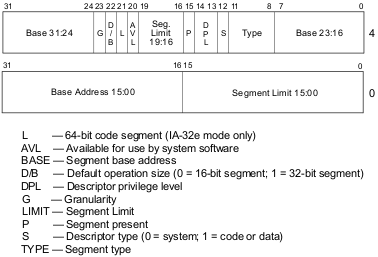
\includegraphics[width=0.5\textwidth]{images/segment_descriptor}
  \caption{Segment Descriptor}
\end{figure}

Luego, cargamos la GDT con el comando \command{lgdt} y el descriptor de la GDT armado desde C (\texttt{GDT\_DESC}).

\subsection{Pasaje a Modo Protegido}
Una vez armada la GDT y habilitado el A20, debemos habilitar Modo Protegido. El modo de protección esta definido por el bit menos significativo del registro \reg{CR0}. Usando un \& con \addr{0x1}, habilitamos este bit.

Una vez que tenemos todas las estructuras necesarias armadas, hay que hacer un \command{jump far} al segmento de código de nivel 0 en la \texttt{GDT}. De esta forma finalmente habilitamos la protección por hardware y pasamos a Modo Protegido. 

